% LaTeX source for ``Algorithms for Computer Simulation of Molecular Systems''
% Copyright (c) 2023 รังสิมันต์ เกษแก้ว (Rangsiman Ketkaew).

% License: Creative Commons Attribution-NonCommercial-NoDerivatives 4.0 International (CC BY-NC-ND 4.0)
% https://creativecommons.org/licenses/by-nc-nd/4.0/

\chapter{กลศาสตร์ควอนตัมเชิงโมเลกุล}
\label{ch:mol_qm}

%----------------------------------------
\section{การจำลองเชิงตัวเลขและเทคนิคเชิงคอมพิวเตอร์}
%----------------------------------------

การจำลองเชิงตัวเลข (Numerical Modeling) คือวิธีที่การที่เราใช้ปัญหาทางคณิตศาสตร์และฟิสิกส์แบบต่าง ๆ เช่น นำมาใช้แก้สมการเชิง%
อนุพันธ์ที่ใช้ในการอธิบายปรากฏการณ์ต่าง ๆ ทางธรรมชาติซึ่งอาจจะมีความยากหรืออาจจะไม่มีทางแก้ได้ด้วยวิธีเชิงวิเคราะห์ (Analytical Method)
\idxboth{การจำลองเชิงตัวเลข}{Numerical Modeling}
\idxboth{วิธีเชิงวิเคราะห์}{Analytical Method}

สำหรับการจำลองด้วยเทคนิคเชิงคอมพิวเตอร์ (Computer Simulation) นั้นเป็นการศึกษาการตอบสนองเชิงพลวัต (Dynamic Response) 
ของระบบแบบจำลองต่อเงื่อนไขเริ่มต้น (Initial Conditions) ที่เราได้กำหนดไว้ โดยเงื่อนไขเริ่มต้นนี้สอดคล้องกับสภาวะจริงของระบบนั้น
\idxboth{เทคนิคเชิงคอมพิวเตอร์}{Computer Simulation}
\idxboth{เงื่อนไขเริ่มต้น}{Initial Conditions}

\begin{figure}[htbp]
    \centering
    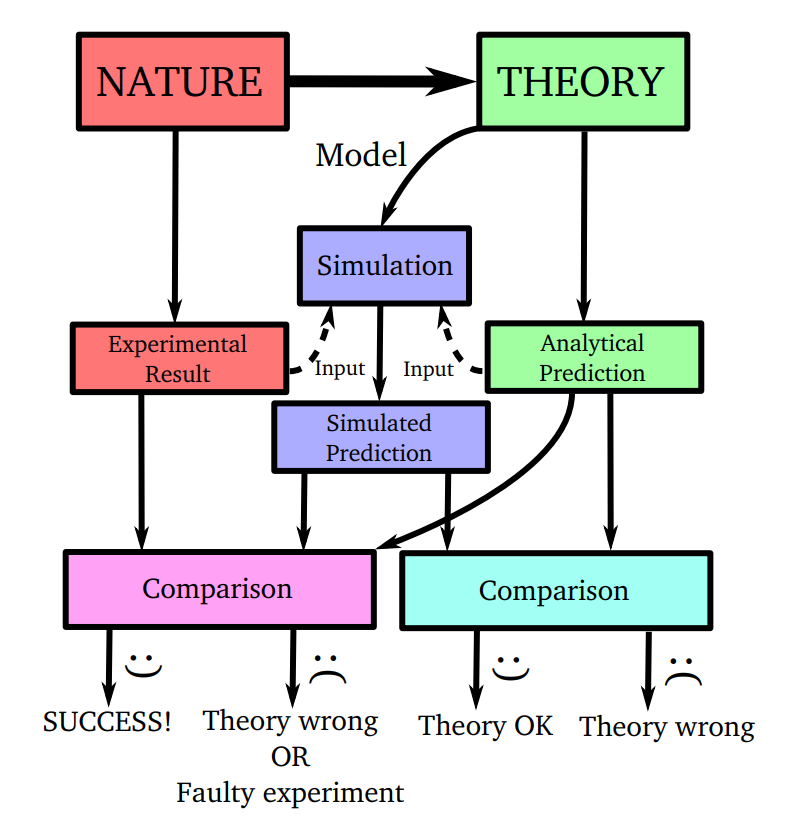
\includegraphics[width=0.8\linewidth]{fig/simulation-modeling-graph.png}
    \label{fig:sim_model_graph}
    \caption{แผนผังความเชื่อมโยงของระบบที่เราต้องศึกษา (Nature), ทฤษฎีหรือวิธีที่ใช้ในการศึกษา (Theory), แบบจำลองหรือโมเดล 
    (Model), ผลการทดลอง (Experimental Result), และผลการคำนวณหรือผลการทำนาย (Computational Results หรือ Prediction)}
\end{figure}

ภาพที่ \ref{fig:sim_model_graph} แสดงแผนผังเชื่อมโยงความแตกต่างระหว่าง Numerical Modeling กับ Computer Simulation 
นั้นก็คือใน Simulation นั้นระบบจำลองของเราจะถูกสร้างขึ้นมา เช่น เราสร้างระบบที่เป็นโมเลกุลน้ำหลาย ๆ โมเลกุลเกาะกลุ่มรวมกัน (Water 
Cluster) โดยเราหวังว่า Water Cluster ที่เราสร้างขึ้นมานี้จะสามารถเป็นตัวแทนของระบบของโมเลกุลน้ำจริง ๆ ได้ ซึ่งก็จะทำให้เราสามารถ%
ศึกษาคุณสมบัติต่าง ๆ ของโมเลกุลน้ำได้ตามต้องการ ส่วนการจำลองเชิงตัวหรือ Numerical Simulation นั้นจะเป็นการสร้างการทดลองเสมือนจริง 
(Virtual Experiments) ของระบบจำลองขึ้นมา อย่างไรก็ตามในบทความวิชาการทางด้านเคมีเชิงคำนวณหรือชีวเชิงคำนวณนั้นเรามักจะพบว่าคำว่า 
Modeling นั้นสามารถถูกแทนด้วยคำว่า Simulation ได้เช่นกัน

คำถามสำคัญที่หลายคนโดยเฉพาะอย่างนักวิทยาศาสตร์ที่ทำงานวิจัยเชิงการทดลองมักจะถามก็คือ \enquote{ทำไมการจำลองทางคอมพิวเตอร์ถึง%
มีความสำคัญ} คำตอบนั้นมีด้วยกันหลายข้อ ผู้เขียนขอสรุปเป็นประเด็นตามนี้ครับ

\begin{enumerate}
    \item การจำลองทางคอมพิวเตอร์นั้นเปรียบเสมือนเป็นสะพานเชื่อมโยงระหว่างทฤษฎีกับการทดลอง
    \item การทำการทดลองบางอย่างนั้นมีค่าใช้จ่ายที่สูงมากและมีความยากเพราะว่าตัวทฤษฎีนั้นซับซ้อนเกินไป ดังนั้นการจำลองทางคอมพิวเตอร์%
    นั้นจะเข้ามาช่วยในการจำลองการทดลองและทดสอบสมมติฐานเพื่อยืนยันทฤษฎีด้วย
    \item การจำลองทางคอมพิวเตอร์นั้นช่วยหาปัจจัยและเงื่อนไขที่เหมาะสมสำหรับการทดลองได้
    \item การจำลองทางคอมพิวเตอร์สามารถแสดงกระบวนการของระบบที่เราสนใจได้ ซึ่งอาจจะทำได้ยากในเชิงการทดลอง
    \item การจำลองทางคอมพิวเตอร์สามารถนำมาใช้ในการศึกษาปรากฏการณ์ที่การทดลองนั้นอาจจะให้ผลการทดลองที่ไม่ละเอียดพอ
\end{enumerate}

อย่างไรก็ตามผู้เขียนต้องขอสรุปเพิ่มเติมด้วยว่าการใช้แบบจำลองทางคอมพิวเตอร์เพียงอย่างเดียวนั้นจะเปล่าประโยชน์ถ้าหากว่าไม่มีผลการทดลองที่%
น่าเชื่อมายืนยันความถูกต้องของผลการคำนวณ ดังนั้นเคมีเชิงการทดลองกับเคมีเชิงคำนวณนั้นจึงเป็นศาสตร์ที่ต้องพึ่งพาอาศัยกัน

%----------------------------------------
\section{Basis Set}
%----------------------------------------

\enquote{Basis Set สำคัญยังไง ทำไมเราต้องกำหนด Basis Set ก่อนการรันการคำนวณเคมีควอนตัมทุกครั้ง?} ผู้เขียนเริ่มต้นหัวข้อด้วยคำถาม%
นี้ก็เพราะว่าผู้อ่านหลายคนน่าจะให้ความสนใจ ใครที่เรียนวิชาเคมีคำนวณ (Electronic structure) หรือกำลังทำงานวิจัยทางด้านนี้อยู่น่าจะต้องเคย%
มีประสบการณ์ในการคำนวณเคมีควอนตัมสำหรับการศึกษาคุณสมบัติของโมเลกุลโดยการใช้วิธีทางควอนตัมกันมาบ้างแล้ว ปกติแล้วเราจะต้องทำการกำหนด 
Basis Set ที่เราจะใช้สำหรับอะตอมแต่ละตัวซึ่งโดยทั่วไปเราก็มักจะเลือก Basis Set เพียงแค่ 1 อันสำหรับทั้งโมเลกุล เช่น 6-31G(d) หรือ cc-pVTZ 
แล้ว Basis Set สำคัญยังไงและส่งผลต่อความถูกต้องของผลที่ได้จากการคำนวณมากน้อยแค่ไหน เราจะมาหาคำตอบกันในหัวข้อนี้

ต้องเท้าความความรู้ที่เราเคยเรียนกันจากวิชากลศาสตร์ควอนตัมเชิงโมเลกุล (Molecular Quantum Mechanics) ก่อนว่าเราใช้ออร์บิทัลเชิงโมเลกุลหรือ 
Molecular Orbitals (MOs) ในการอธิบายโมเลกุลซึ่ง MOs นี้สามารถถูกเขียนให้อยู่ในรูปของผลรวมเชิงเส้นของออร์บิทัลเชิงอะตอมหรือ Atomic 
Orbitals (AOs) ได้หรือที่เรียกว่าวิธี Linear Combination of Atomic Orbitals (LCAO) ซึ่งก็มาจากแนวคิดที่ว่าอะตอมหลาย ๆ อะตอม%
รวมกันได้เป็นโมเลกุล

\begin{equation}
    \label{eq:mo_lcao}
    \psi_{i} = \sum_{j} c_{ij} \varphi_{j}
\end{equation}

ในการเขียนสมการคณิตศาสตร์เพื่ออธิบายออร์บิทัลนั้นโดยทั่วไปแล้วเรามักจะเขียนด้วยตัวอักษรกรีก ตัวอย่างเช่นเราใช้ psi ($\psi$) ในการแทน MOs 
และใช้ phi ($\varphi$) ในการแทน Basis Function ซึ่งเราสามารถเขียน MOs ได้ด้วยวิธี LCAO ซึ่งเป็นผลรวมของผลคูณระหว่างสัมประสิทธิ์ $c$ 
กับ Basis Function สำหรับแต่ละ MOs ในโมเลกุล จริง ๆ แล้ว $c$ นั้นมีชื่อเต็ม ๆ ว่า \enquote{สัมประสิทธิ์การกระจายของออร์บิทัลเชิงโมเลกุล} 
หรือ Molecular Orbital Expression Coefficients หรือเราจะเรียกสั้น ๆ ว่า MO Coefficients ก็ได้ 

ในทางทฤษฎีนั้น Basis Function จะถูกกำหนดให้มีตำแหน่งอยู่ที่จุดศูนย์กลางของอะตอม (Atom-centered Basis Function) อย่างไรก็ตามเรา%
ไม่มีกฎตายตัวว่า Basis Function นั้นจะต้องอยู่จุดศูนย์กลางของอะตอมเสมอไปถ้าหากเราสามารถหาฟังก์ชันที่อธิบายรูปร่างของออร์บิทัลได้อย่างเหมาะสม
คราวนี้เราจะมาดูรายละเอียดของ Basis Function โดยผมขอยกตัวอย่างของ Basis Set ที่ได้รับความนิยมมาก ๆ อันหนึ่งนั่นก็คือ 6-31G(d) 
ซึ่งหลาย ๆ คนมักจะใช้กันตอนที่เตรียม Input File สำหรับรันการคำนวณ เราจะมาดูรายละเอียดประเภทของฟังก์ชันที่เป็นหน้าตาของ Basis Function 
กันก่อน ในช่วงยุคเริ่มต้นของการพัฒนาวิธีสำหรับการคำนวณ Electronic Structure นั้นได้มีการพัฒนาสิ่งที่เรียกว่า Slater Type Orbitals 
(STOs) ขึ้นมา ซึ่ง STOs นี้เป็นฟังก์ชันที่ถูกสร้างขึ้นมาจากการนำฟังก์ชัน 2 ฟังก์ชันมารวมกันนั่นคือฟังก์ชันของส่วนเป็นเชิงรัศมี (Radial Part) 
กับฟังก์ชันของส่วนที่เป็นเชิงมุม (Angular Part) ที่อธิบายรัศมีหรือขนาดของออร์บิทัลและอธิบายรูปร่างของออร์บิทัลตามลำดับ สมการของ STOs คือ

\begin{equation}
    \label{eq:sto}
    R(r) = N r^{n - 1} e^{-\zeta r}
\end{equation}

เมื่ออ่านมาถึงจุดนี้แล้วผู้อ่านก็น่าจะเข้าใจได้ทันทีเลยว่า STOs นั้นก็คือฟังก์ชันเริ่มต้นที่ถูกนำมาใช้ในการอธิบายออร์บิทัลหรือฟังก์ชันคลื่น (Wavefunction) 
ของอิเล็กตรอนที่อยู่ในอะตอมนั้น ๆ ขึ้นมา ถ้าหากเราพลอต STOs Function ให้เป็นฟังก์ชันกับรัศมีแล้วเราจะได้ฟังก์ชันที่มันจะมีความราบเรียบ (Smooth) 
ตามค่ารัศมีที่เพิ่มขึ้น อย่างไรก็ตามการใช้ STOs นั้นมีข้อจำกัดหรือข้อด้อยสำหรับการนำไปใช้ในการคำนวณก็คือเทอมที่เป็น Two-electron Integral 
หรือ Electron Repulsion Integral (ERI) ที่ถูกอินทิเกรตโดยใช้ STOs นั้นคำนวณได้ยากมาก ๆ ดังนั้นในช่วงเวลาต่อมาจึงได้มีการพัฒนาฟังก์ชัน%
ที่เหมือนกับว่าคล้าย ๆ กับ STOs ขึ้นมาแต่สามารถนำไปใช้ได้ในกรณีที่หลากหลายกว่า (General) นั่นก็คือ Gaussian Type Orbitals (GTOs) 
ซึ่งก็ตามชื่อเลยนั่นคือฟังก์ชันที่ใช้เป็น Gaussian Function โดยมีสมการคือ

\begin{equation}
    \label{eq:gto}
    G_{nlm} (r, \theta , \psi ) = N_n \underbrace{r^{n-1} e^{-\alpha r^2}}_{\text{radial part}} 
    \underbrace{Y^m_l (\theta, \psi)}_{\text{angular part}}
\end{equation}

ความแตกต่างระหว่าง STOs กับ GTOs ก็คือเทอมที่เป็นดีกรีหรือกำลังของฟังก์ชัน Exponential ใน GTOs นั้นเราจะมีการนำรัศมีมายกกำลัง ($r^{2}$) 
แต่ว่าใน STOs นั้นรัศมีจะเป็นแค่กำลังหนึ่งเท่านั้น GTOs นั้นมีประโยชน์มาก ๆ ในการคำนวณเพราะว่าเราสามารถคำนวณ ERI ได้ง่ายกว่า STO มาก 
ผู้อ่านที่สนใจรายละเอียดของทฤษฎีสามารถอ่านบทความวิชาการของ S.F. Boys ที่ตีพิมพ์งานวิจัยในปี 1950 หรือประมาณ 70 ปีที่แล้วได้ ผมขอสรุป%
อย่างนี้ครับว่าความแตกต่างระหว่าง STOs กับ GTOs นั้นก็คือลักษณะพฤติกรรมของตัวฟังก์ชันที่ $r = 0$ (ที่จุดศูนย์กลางของอะตอม) กับที่ $r = \inf$ 
(Infinity) หรือที่ใกลจากนิวเคลียสมาก ๆ โดยที่ STOs นั้นจะมี Cusp หรือจุดที่เป็นการเปลี่ยนหรือ Transition ระหว่าง States ที่ตำแหน่ง 
$r = 0$ ในขณะที่ GTOs นั้นจะมีความไม่ถูกต้องที่ตำแหน่ง $r = 0$ นอกจากนี้คือลักษณะของฟังก์ชัน GTO จะมีค่าที่ลดลงเร็วกว่า STO มากโดย%
เฉพาะตำแหน่งที่อิเล็กตรอนนั้นอยู่ห่างจากนิวเคลียสแบบไกล ๆ ($r = \inf$) นอกจากนี้แล้วยังมีฟังก์ชันแบบพิเศษอีกอันนึงที่เรียกว่า Contracted 
Gaussian Type Orbitals ด้วยซึ่งเป็นการปรับปรุงให้ GTOs สามารถอธิบายพฤติกรรมของอิเล็กตรอนสำหรับออร์บิทัลเชิงอะตอมได้ดียิ่งขึ้น

กลับมาที่คำถามของเรานั่นก็คือ Basis Set สำคัญยังไง คำตอบคือ Basis Set นั้นจะประกอบไปด้วยข้อมูลที่เราจะนำมาใช้ในการสร้าง MOs นั่นเอง 
โดยที่ในไฟล์หนึ่งไฟล์นั้นจะมีข้อมู, เช่น ประเภทของออร์บิทัล (Orbital Types), จำนวนของ Primitive Gaussian, Scale Factor, Orbital 
Exponent และที่สำคัญคือ Coefficients ที่จะถูกนำมาใช้ในการสร้าง Wavefunction เริ่มต้นนั่นเอง โดยฟอร์แมทของ Basis Set ในไฟล์นั้นมีดังนี้

\begin{verbatim}
atomic symbol
Shell_type, No. of primitive Gaussians, Scale_factor
Orbital exponent, Contraction coefficient
[repeat x times]
\end{verbatim}

โดยที่ $x$ คือจำนวนของ Primitive Gaussian ตัวอย่างเช่น Basis Set "STO-3d" ของอะตอมคาร์บอนนั้นมีดังนี้

\begin{verbatim}
C 0
S 3 1.00
.7161683735D+02 .1543289673D+00
.1304509632D+02 .5353281423D+00
.3530512160D+01 .4446345422D+00
SP 3 1.00
.2941249355D+01 -.9996722919D-01 .1559162750D+00
.6834830964D+00 .3995128261D+00 .6076837186D+00
.2222899159D+00 .7001154689D+00 .3919573931D+00
\end{verbatim}
    
เราจะมาดูทีละแถวกัน 

\begin{itemize}
    \item แถวแรกคือระบุว่าเป็นออร์บิทัล 1s ของอะตอมคาร์บอนซึ่งสามารถเขียนได้ด้วยผลรวมของ Primitive Gaussian 3 อันโดยมีตัวคูณปรับ%
    ขนาด (Scale Factor) คือ 1
    \item แถวที่ 2-4 คือเป็น Orbital exponent และ  coefficients ตามลำดับ 
\end{itemize}

\noindent ดังนั้นสำหรับออร์บิทัล 1s ของอะตอมคาร์บอนนั้นจะมาสามารถเขียนได้เป็นผลรวมของเทอม STO Functions 3 ฟังก์ชันรวมกันนั่นเอง 
สำหรับออร์บิทัลอื่น ๆ ของอะตอมคาร์บอนนั้นก็ทำแบบเดียวกันแต่ว่าจะมีเทคนิคบางอย่างมาช่วยให้การคำนวณนั้นทำได้เร็วขึ้น เช่น ออร์บิทัล 2s กับ 2p 
นั้นจะใช้ Orbital Exponent ค่าเดียวกันแต่ว่าจะใช้ Contraction Coefficients ที่ต่างกัน คราวนี้เราลองมาทำแบบฝึกหัดสั้น ๆ ในการนับจำนวน%
ของ Basis Functions ที่เราต้องการนำมาใช้สำหรับโมเลกุล Methanol (\ce{CH4O}) กัน เริ่มต้นเลยสำหรับ AOs 1s, 2s, และ 2p นั้นเราจะใช้ 
Gaussian 3 ฟังก์ชัน ดังนั้นเราจะมี Basis Function 5 อันสำหรับคาร์บอนแต่ละอะตอมและสำหรับอะตอมออกซิเจนด้วย และจะมีแค่ Basis Function 
1 ฟังก์ชันสำหรับอะตอมไฮโดรเจนแต่ละตัว ดังนั้นรวมทั้งหมดเราจะมี 14 Basis Functions ซึ่งก็เท่ากับ 14 MO-coefficients สำหรับการทำ SCF 
Calculation ในแต่ละรอบนั่นเอง คราวนี้ Basis Function ทั้ง 14 อันนั้นจะมี Gaussian Primitive อีก 3 อันย่อย ดังนั้นจำนวน Primitives 
ทั้งหมดของโมเลกุล \ce{CH4O} จึงเท่ากับ $14 \time 3 = 42 $ 

สำหรับการคำนวณจำนวน Basis Function และ Gaussian Primitive นั้นมีรายละเอียดอีกเยอะพอสมควร ขึ้นอยู่กับว่าใช้ Basis Set แบบไหน 
เพราะว่า Basis Set นั้นมีหลายประเภท เช่น Split-valence, Double Zeta, Polarization, หรือ Diffuse Functions นอกจากนี้การ%
เลือกใช้ Basis Set นั้นก็ขึ้นอยู่กับประเภทของโมเลกุลรวมถึงสิ่งที่ต้องการคำนวณด้วย
